\chapter{Решение уравнений с монотонным оператором}
В первой главе рассматриваются методы решения некорректных задач с монотонным оператором. В рамках двухэтапного подхода, где на первом этапе происходит регуляризация по Лаврентьеву, на втором этапе решения задачи применяются регуляризованные алгоритмы. Первый параграф главы посвящен вопросам сходимости регуляризованного метода Ньютона. Второй параграф содержит схемы построения итерационных процессов градиентного типа --- нелинейных $\alpha$-процессов и доказывается их сходимость. В третьем параграфе иллюстрируются особенности применения рассмотренных в данной главе итерационных методов к нелинейному интегральному уравнению и приводятся результаты численного моделирования.

\newpage
\section{Метод Ньютона}
Рассматривается нелинейное уравнение
\begin{equation}\label{equ1}A(u)=f\end{equation}
в гильбертовом пространстве $U$ с монотонным непрерывно дифференцируемым по Фреше оператором $A$, для которого обратные операторы $A'(u)^{-1}$, $A^{-1}$ разрывны, что влечет некорректность задачи $\eqref{equ1}$. Для построения регуляризующего алгоритма (РА) используется двухэтапный метод, в котором на первом этапе используется регуляризация по схеме Лаврентьева
\begin{equation}\label{equ2}A(u)+\alpha(u-u^0)-f_\delta=0,\end{equation}
где $\|f-f_\delta\|\le\delta$, $u_0$ --- некоторое приближение к решению; а на втором этапе для аппроксимации регуляризованного решения $u_\alpha$ применяется регуляризованный метод Ньютона (РМН)
\begin{equation}\label{equ_rmn}
u^{k+1}=u^k-\gamma(A'(u^k)+\bar\alpha I)^{-1}(A(u^k)+\alpha(u^k-u^0)-f_\delta)\equiv{T(u^k)}.
\end{equation}
Здесь $\alpha, \bar\alpha$ --- положительные параметры регуляризации, $\gamma>0$ --- демпфирующий множитель (параметр регулировки шага).

Так как оператор $A$ --- монотонный, то его производная $A'(u^k)$ --- неотрицательно определенный оператор. Следовательно, операторы $(A'(u^k)+\bar\alpha I)^{-1}$ существуют и ограничены, следовательно, процесс $\eqref{equ_rmn}$ определен корректно.

Ранее в рамках двухэтапного подхода в работах В.В. Васина и авторов \cite{VasAkiMin2013, Vasin2014} исследовался модифицированный метод Ньютона, когда вместо $A'(u^k)$ в $\eqref{equ_rmn}$ используется производная в начальной точке $A'(u^0)$ в ходе всего итерационного процесса, где $A'(u^0)$ --- самосопряженный неотрицательно определенный оператор.  

Пусть имеются следующие условия
\begin{equation}\label{cond1.1}
\|A(u)-A(v)\|\le N_1\|u-v\|, \quad \forall u, v \in U,
\end{equation}
\begin{equation}\label{cond1.2}
\|A'(u)-A'(v)\|\le N_2\|u-v\|, \quad \forall u, v \in U.
\end{equation}
и известна оценка для нормы производной в точке $u^0$ (начальном приближении), т.е.
\begin{equation}\label{cond1.3}
\|A'(u^0)\| \le N_0\le N_1, \quad \|u^0-u_\alpha\| \le r.
\end{equation}
\mbox{З\ а\ м\ е\ ч\ а\ н\ и\ е 1.1.} Начальное приближение в неравенстве $\eqref{cond1.3}$ в общем случае не обязано совпадать с $u^0$ в схеме $\eqref{equ2}$. Однако, для простоты изложения, будем считать, что это один и тот же элемент. Кроме того, для монотонного оператора $A$ оператор $A+\alpha I$ --- равномерно монотонный, поэтому при выполнении условия $\ref{cond1.1}$ согласно [\cite{KufFuch1988},~теорема 43.7], регуляризованное уравнение (\ref{equ2}) имеет единственное решение.

\begin{theorem}\label{teo2.1} Пусть $A$ --- монотонный оператор, для которого выполнены условия $\eqref{cond1.1}$, $\eqref{cond1.2}$ для $u, v \in S_r(u_\alpha)$, $r\le \alpha/N_2$, $0<\alpha \le \bar\alpha$, $u^0 \in S_r(u_\alpha)$. 
	
	Тогда для процесса $\eqref{equ_rmn}$ c $\gamma=1$ имеет место линейная скорость сходимости метода при аппроксимации единственного решения $u_\alpha$ регуляризованного уравнения $\eqref{equ2}$
	\begin{equation}\label{nwt_conv}
	\| u^k-u_\alpha \| \le q^kr, \quad q=(1-\frac{\alpha}{2\bar\alpha}).
	\end{equation}
\end{theorem}
\proof 
Учитывая, что для монотонного оператора $A$ $\| (A'(u)+\bar\alpha I)^{-1} \| \le 1/\bar\alpha$, а из $\eqref{cond1.2}$ следует справедливость разложения
$$
A(u_\alpha)=A(u^k)+A'(u^k)(u_\alpha-u^k)+\xi, \quad \|\xi\|\le \frac{N_2}{2}\|u_\alpha-u^k\|^2,
$$
приходим к соотношению 
$$
u^{k+1}-u_\alpha=u^k-u_\alpha-(A'(u^k)+\bar\alpha I)^{-1}(A(u^k)-A(u_\alpha)+\alpha(u^k-u_\alpha))=u^k- u_\alpha$$ $$-(A'(u^k)+\bar\alpha I)^{-1}(A'(u^k)(u^k-u_\alpha)+\bar\alpha(u^k-u_\alpha)-\xi+(\alpha-\bar\alpha)(u^k-u_\alpha)). $$
Из полученного соотношения вытекает оценка
$$
\|u^{k+1}-u_\alpha\|\le\frac{1}{\bar\alpha}\left(\frac{N_2{\|u^{k}-u_\alpha\|}^2}{2}+(\bar\alpha-\alpha)\|u^k-u_\alpha\|\right)$$
$$\le\left(1-\frac{\alpha}{\bar\alpha}+\frac{N_2}{2\bar\alpha}\|u^k-u_\alpha\|\right)\|u^k-u_\alpha\|.$$
Имея $\|u^0-u_\alpha\|\le r \le \alpha/N_2$ и предполагая $\| u^{k}-u_\alpha \|\le q^kr$, по индукции приходим к оценке $\eqref{nwt_conv}$.

Усиленное свойство Фейера [\cite{VasEre2009}, определение 1.3] для оператора $T$ означает, что для некоторого $\nu>0$ выполнено соотношение
\begin{equation}\label{fejer_prop_uni}
{\|T(u)-z\|}^2\le{\|u-z\|}^2-\nu{\|u-T(u)\|}^2,
\end{equation}
где $z\in Fix(T)$ --- множество неподвижных точек оператора $T$. Это влечет для итерационных точек $u^k$, порождаемых процессом $u^{k+1}=T(u^k)$, выполнение неравенства
\begin{equation}\label{fejer_prop_it}
{\|u^{k+1}-z\|}^2\le{\|u^k-z\|}^2-\nu{\|u^k-u^{k+1}\|}^2.
\end{equation}
Важным свойством фейеровских операторов является замкнутость относительно операций произведения и взятия выпуклой суммы. Располагая итерационными процессами с фейеровским оператором шага и общим множеством неподвижных точек, можно конструировать разнообразные гибридные методы, а также учитывать в итерационном алгоритме априорные ограничения на решение в виде системы линейных или выпуклых неравенств.

Установим усиленное свойство Фейера для оператора шага $T$ в методе $\eqref{equ_rmn}$.
\begin{theorem}\label{teo2.2} Пусть для монотонного оператора $A$ выполнены условия $\eqref{cond1.1}$ --- $\eqref{cond1.3}$, $A'(u^0)$ --- самосопряженный оператор, $\|u_\alpha-u^0\|\le r$ и для параметров справедливы соотношения 
	\begin{equation}\label{cond2.7}
	0\le\alpha\le\bar\alpha,\quad\bar\alpha\ge 4N_1,\quad r\le\alpha/8N_2.
	\end{equation}
	Тогда для оператора
	$$ F(u)=(A'(u)+\bar\alpha I)^{-1}(A(u)+\alpha(u-u^0)-f_\delta) $$
	справедлива оценка снизу
	\begin{equation}\label{est2.8}
	\langle F(u), u-u_\alpha\rangle\ge\frac{\alpha}{4\bar\alpha}{\|u-u_\alpha\|}^2 \quad \forall u \in S_r(u_\alpha).
	\end{equation}
\end{theorem}
\proof Введем обозначение $B(u)=A'(u)+\bar\alpha I$. Принимая во внимание, что $u_\alpha$ --- решение уравнения $\eqref{equ2}$, имеем
$$
\langle F(u), u-u_\alpha\rangle=\langle F(u)-F(u_\alpha), u-u_\alpha\rangle=\alpha\langle B^{-1}(u)(u-u_\alpha), u-u_\alpha\rangle$$ \begin{equation}\label{ineq2.9}+\langle B^{-1}(u)(A(u)-A(u_\alpha)), u-u_\alpha\rangle.
\end{equation}
Учитывая, что $A'(u^0)$ --- самосопряженный и, ввиду монотонности $A$, неотрицательно определенный оператор, для первого слагаемого в правой части равенства $\eqref{ineq2.9}$, получаем
$$\alpha\langle B^{-1}(u)(u-u_\alpha), u-u_\alpha\rangle=\alpha\langle B^{-1}(u^0)(u-u_\alpha), u-u_\alpha\rangle$$ $$+\alpha\langle (B^{-1}(u)-B^{-1}(u^0))(u-u_\alpha), u-u_\alpha\rangle \ge \frac{\alpha}{\bar\alpha+N_0}{\|u-u_\alpha\|}^2$$
$$ - \alpha|\langle B^{-1}(u)(B(u^0)-B(u))B^{-1}(u^0)(u-u_\alpha), u-u_\alpha\rangle| $$
$$\ge \left( \frac{\alpha}{\bar\alpha+N_0}-\frac{\alpha N_2\|u-u^0\|}{{\bar\alpha}^2}\right)\|u-u_\alpha\|^2$$
\begin{equation}\label{ineq2.10}
\ge\left(\frac{\alpha}{\bar\alpha+N_0}-\frac{2\alpha N_2r}{{\bar\alpha}^2}\right)\|u-u_\alpha\|^2,
\end{equation} где использовано неравенство $\|u-u^0\|\le\|u-u_\alpha\|+\|u_\alpha-u^0\|\le 2r$.
Для второго слагаемого в правой части $\eqref{ineq2.9}$ имеем
$$ \langle B^{-1}(u)(A(u)-A(u_\alpha)), u-u_\alpha\rangle= \langle B^{-1}(u^0)(A(u)-A(u_\alpha)), u-u_\alpha\rangle$$
$$+\langle (B^{-1}(u)-B^{-1}(u^0))(A(u)-A(u_\alpha)), u-u_\alpha\rangle$$
$$=\langle B^{-1}(u^0)\int\limits_0^1 (A'(u_\alpha+\theta(u-u_\alpha))-A'(u^0))d\theta (u-u_\alpha), u-u_\alpha\rangle$$
$$+ \langle B^{-1}(u^0)A'(u^0)(u-u_\alpha), u-u_\alpha\rangle $$
$$+\langle (B^{-1}(u)-B^{-1}(u^0))(A(u)-A(u_\alpha)), u-u_\alpha\rangle$$
$$\ge-\frac{N_2}{\bar\alpha}\int\limits_0^1\|u_\alpha+\theta(u-u_\alpha)-u^0\|d\theta {\|u-u_\alpha\|}^2 $$
$$-\frac{1}{{\bar\alpha}^2}\left ( \|A'(u)-A'(u^0)\|\|A(u)-A(u_\alpha)\|\|(u-u_\alpha)\|\right ) $$$$ \ge - \frac{N_2}{2\bar\alpha} \left ( \|u_\alpha-u^0\|+\|u-u^0\|\right ){\|u-u_\alpha\|}^2 - \frac{N_1 N_2}{{\bar\alpha}^2}\|u-u^0\| {\|u-u_\alpha\|}^2 $$
\begin{equation}\label{ineq2.11}
\ge -\frac{3N_2r}{2\bar\alpha}{\|u-u_\alpha\|}^2-\frac{2rN_1 N_2}{{\bar\alpha}^2}{\|u-u_\alpha\|}^2.\end{equation}

Объединяя $\eqref{ineq2.10}$,$\eqref{ineq2.11}$, приходим к неравенству $$
\langle F(u), u-u_\alpha\rangle\ge\left (\frac{\alpha}{\bar\alpha+N_0}-\frac{2N_2 r \alpha}{{\bar\alpha}^2}-\frac{3N_2r}{2\bar\alpha}-\frac{2rN_1 N_2}{{\bar\alpha}^2}\right ){\|u-u_\alpha\|}^2, $$ откуда с учетом условий $\eqref{cond2.7}$ на параметры $\alpha$, $\bar\alpha$, $r$, а также неравенства $N_1\ge N_0$, приходим к оценке $\eqref{est2.8}$.
\begin{theorem} \label{teo2.3} 
	Пусть выполнены условия теоремы $\ref{teo2.2}$. Тогда при
	\begin{equation}\label{ineq2.12}
	\gamma<\frac{\alpha\bar\alpha}{2(N_1+\alpha)^2}
	\end{equation}
	оператор шага $T$ процесса $\eqref{equ_rmn}$ при
	\begin{equation}\label{eq2.13}
	\nu=\frac{\alpha\bar\alpha}{2\gamma(N_1+\alpha)^2}-1
	\end{equation}
	удовлетворяет неравенству $\eqref{fejer_prop_uni}$, для итераций $u^k$ справедливо соотношение $\eqref{fejer_prop_it}$ и имеет место сходимость
	\begin{equation}\label{eq2.14}
	\lim_{k\to\infty}\|u^k-u_\alpha\|=0.
	\end{equation}
	Если параметр $\gamma$ принимает значение \begin{equation}\label{eq2.15}
	{\gamma}_{opt}=\frac{\alpha\bar\alpha}{4(N_1+\alpha)^2},
	\end{equation} то справедлива оценка \begin{equation}\label{est2.16}
	\|u^k-u_\alpha\|\le q^k r, \quad q=\sqrt{1-\frac{{\alpha}^2}  {16(N_1+\alpha)^2}}.\end{equation}
\end{theorem}
\proof В условиях теоремы справедливо неравенство
\begin{equation}\label{eq2.17}
\|F(u)\|^2\le\|B^{-1}(u)\|^2\|A(u)-A(u_\alpha)+\alpha(u-u_\alpha)\|^2 \le \frac{(N_1+\alpha)^2}{\bar\alpha^2}{\|u-u_\alpha)\|}^2,
\end{equation}
которое вместе с $\eqref{est2.8}$ влечет соотношение
\begin{equation}\label{ineq2.18}
{\|F(u)\|}^2 \le \frac{4(N_1+\alpha)^2}{\alpha\bar\alpha}\langle F(u), u-u_\alpha\rangle.
\end{equation}
Условие $\eqref{fejer_prop_uni}$ на оператор шага $T$ эквивалентно 
\begin{equation}\label{ineq2.19}
{\|F(u)\|}^2 \le \frac{2}{\gamma(1+\nu)}\langle F(u), u-u_\alpha\rangle.
\end{equation}
Сравнивая неравенства $\eqref{ineq2.18}$ и $\eqref{ineq2.19}$, получаем условие $\eqref{ineq2.12}$ для $\gamma$ и выражение $\eqref{eq2.13}$ для $\nu$.

При $u=u^k$ из неравенства $\eqref{fejer_prop_uni}$ вытекает $\eqref{fejer_prop_it}$ и соотношение
$$ \|u^k-T(u^k)\|=\gamma\|F(u^k)\|\to 0, \quad k\to\infty,$$ что вместе с $\eqref{est2.8}$ влечет сходимость $\eqref{eq2.14}$.
Принимая во внимание $\eqref{est2.8}$, $\eqref{eq2.17}$, имеем неравенство
$$ {\|u^{k+1}-u_\alpha\|}^2={\|u^k-u_\alpha\|}^2-2\gamma\langle F(u^k), u^k-u_\alpha\rangle+{\gamma}^2\|F(u^k)\|^2 $$
\begin{equation}\label{ineq2.20}
\le \left (1-\gamma\frac{\alpha}{2\bar\alpha}+{\gamma}^2\frac{(N_1+\alpha)^2}{{\bar\alpha}^2}\right )\|u^k-u_\alpha\|^2
\end{equation}
При значениях $\gamma={\gamma}_{opt}$ из $\eqref{eq2.15}$ выражение в круглых скобках неравенства $\eqref{ineq2.20}$ достигает минимума и при $\gamma={\gamma}_{opt}$ параметр $q$ вычисляется по формуле, представленной в $\eqref{est2.16}$.

\newpage
\section{Нелинейные альфа-процессы}
Для решения уравнения $\eqref{equ2}$ могут применяться методы градиентного типа, которые мы назовем нелинейными $\alpha$-процессами
\begin{equation}\label{equ_alphaproc}
u^{k+1}=u^k-\gamma\frac{\langle (A'(u^k)+\bar\alpha I)^{\varkappa}S_\alpha(u^k), S_\alpha(u^k)\rangle }{\langle(A'(u^k)+\bar\alpha I)^{\varkappa+1}S_\alpha(u^k), S_\alpha(u^k)\rangle }S_\alpha(u^k)\equiv{T(u^k)}
\end{equation}
при $\varkappa=-1,0,1$. Здесь $\alpha, \bar\alpha$ --- положительные параметры регуляризации, $\gamma>0$ --- параметр регулировки шага, $S_\alpha(u)=A(u)+\alpha(u-u^0)-f_\delta$.

Сначала опишем экстремальные принципы, которые используются при построении процессов $\eqref{equ_alphaproc}$ для нелинейного монотонного оператора $A$. Используя разложение Тейлора в точке $u^k$ и удерживая лишь два члена, приходим к линейному уравнению
\begin{equation*}
A(u^k)+A'(u^k)(u-u^k)=f_{\delta}.
\end{equation*}
Зададим итерационный процесс в следующем виде
\begin{equation*}
u^{k+1}=u^k-\beta(A(u^k)-f_{\delta})
\end{equation*}
и найдем параметр $\beta$ из условия
\begin{equation}\label{cond3.1}
\min_{\beta}{\|u^k-\beta(A(u^k)-f_{\delta})-z\|^2},
\end{equation}
где $z$ --- решение уравнения $A'(u^k)z=F^k$, $F^k=f_{\delta}+A'(u^k)u^k-A(u^k)$. Заменяя теперь оператор $A(u)$ на $A(u)+\alpha(u-u^0)$, а $A'(u^k)$ на $A'(u^k)+\bar\alpha I$, получаем процесс $\eqref{equ_alphaproc}$ при $\varkappa=-1$ и $\gamma=1$, т.е. нелинейный регуляризованный вариант ММО. Если теперь вместо $\eqref{cond3.1}$ использовать экстремальные принципы
$$\min_{\beta}\{\langle A'(u^k)u^{k+1},u^{k+1}\rangle-2\langle u^{k+1},F(u^k)\rangle\},$$
либо 
\begin{equation}\label{cond3.2}
\min_{\beta}\{\|A'(u^k)(u^k-\beta(A(u^k)-f_{\delta})-F(u^k)\|^2\},
\end{equation}
то получаем после тех же замен нелинейный регуляризованный аналог МНС, т.е. $\eqref{equ_alphaproc}$ при $\varkappa=0$ и $\gamma=1$, либо ММН, т.е. $\eqref{equ_alphaproc}$ при $\varkappa=1$, $\gamma=1$ с учетом следующего замечания.

\mbox{З\ а\ м\ е\ ч\ а\ н\ и\ е 1.2.} Формула $\eqref{equ_alphaproc}$ при $\varkappa=1$ справедлива лишь для самосопряженного оператора $A'(u)$. В общем же случае, знаменатель дроби при $\varkappa=1$ следует заменить на $\|(A'(u)+\alpha I)S_\alpha (u)\|^2$, как это следует из условия минимума задачи $\eqref{cond3.2}$. Это обстоятельство будет учтено во всех выкладках в главах 1, 2.

Установим сходимость процесса $\eqref{equ_alphaproc}$ при $\varkappa=-1,0,1$ к решению уравнения $\eqref{equ2}$. Как и прежде, используем обозначения: \begin{equation*}B(u)=A'(u)+\bar\alpha I, \quad S_\alpha (u)=A(u)+\alpha(u-u^0)-f_\delta,\end{equation*}
а также введем новое
$$\beta ^\varkappa =\frac{\langle B^\varkappa(u)S_\alpha(u), S_\alpha (u)\rangle}{\langle B^{\varkappa +1}(u)S_\alpha(u), S_\alpha(u)\rangle}, \quad F^\varkappa(u)=\beta^\varkappa S_\alpha(u), $$ где при $\varkappa=1$ в $\beta^\varkappa$ следует заменить знаменатель на $\|B(u)S_\alpha(u)\|^2$ (см. замечание 1.2).
\begin{theorem}\label{teo3.1}
	Пусть для монотонного оператора $A$ выполнены условия $\eqref{cond1.1}$ --- $\eqref{cond1.3}$ и $A'(u^0)$ --- самосопряженный оператор. Кроме того, для ММО параметры $\alpha$, $\bar\alpha$, $r$, $N_2$, $N_0$ удовлетворяют дополнительным соотношениям:
	\begin{equation}\label{cond3.3}
	\alpha \le \bar\alpha, \quad r\le \alpha/8N_2, \quad \bar\alpha \ge N_0.
	\end{equation}
	Тогда справедливы соотношения
	\begin{equation}\label{ineq3.4}
	\|F^\varkappa(u)\|^2 \le \mu_\varkappa\langle F^\varkappa(u), u-u_\alpha\rangle, \quad \varkappa=-1,0,1,
	\end{equation} где
	\begin{equation}\label{cond3.5}
	\mu _{-1}=\frac{4(N_1+\alpha)^2}{\alpha\bar\alpha}, \quad \mu _0= \frac{(N_1+\alpha)^2(N_1+\bar\alpha)}{\alpha{\bar\alpha}^2}, \quad \mu_1= \frac{(N_1+\alpha)^2(N_1+\bar\alpha)^2}{\alpha{\bar\alpha}^3},
	\end{equation}
	соответственно для ММО, МНС, ММН.
\end{theorem}
\proof Рассмотрим  ММО, т.е. $\eqref{equ_alphaproc}$ при $\varkappa=-1$. Принимая во внимание монотонность оператора $A$, самосопряженность и неотрицательность $A'(u^0)$ и условия на параметры $\eqref{cond3.3}$, имеем (ниже $F^{-1}(u)$, $B^{-1}(u)$, означает $F^\varkappa(u)$, $B^\varkappa(u)$ при $\varkappa=-1$) имеем
$$ \langle F^{-1}(u), u-u_\alpha\rangle=\beta^{-1}(u)\langle A(u)-A(u_\alpha)+ \alpha(u-u_\alpha),u-u_\alpha\rangle\ge\alpha\beta^{-1}(u)\|u-u_\alpha\|^2
$$ $$\ge\alpha\left(\frac{\langle B^{-1}(u^0)S_\alpha(u), S_\alpha(u)\rangle}{\|S_\alpha (u)\|^2}-\frac{\mid\langle (B^{-1}(u)-B^{-1}(u^0))S_\alpha(u), S_\alpha (u)\rangle \mid}{\|S_\alpha (u)\|^2}\right)$$
$$\times \|u-u_\alpha\|^2 \ge\left(\frac{\alpha}{N_0+\bar\alpha}-\alpha\|B^{-1}(u)\|\|B^{-1}(u^0)\|\|A'(u)-A'(u^0)\|\right)\|u-u_\alpha\|^2$$ 
\begin{equation}\label{ineq3.6}
\ge\left(\frac{\alpha}{N_0+\bar\alpha}-\frac{2\alpha N_2r}{\bar\alpha ^2}\right)\|u-u_\alpha\|^2\ge\frac{\alpha}{4\bar\alpha}\|u-u_\alpha\|^2,\end{equation}
где учтено, что $\|u-u^0\|\le\|u-u_\alpha\|+\|u_\alpha-u^0\|\le 2r.$ Кроме того, выполнены неравенства $$\|F^{-1}(u)\|^2=\mid\beta^{-1}(u)\mid^2\|A(u)-A(u_\alpha)+\alpha(u-u_\alpha)\|^2\le(N_1+\alpha)^2\|B^{-1}(u)\|^2\|u-u_\alpha\|^2 $$
\begin{equation}\label{ineq3.7}
\le\frac{(N_1+\alpha)^2}{\bar\alpha^2}\|u-u_\alpha\|^2 .
\end{equation}
Объединяя $\eqref{ineq3.6}$ и $\eqref{ineq3.7}$, получаем
\begin{equation}\label{ineq3.8}
\|F^{-1}(u)\|^2\le\frac{4(N_1+\alpha)^2}{\alpha\bar\alpha}\langle F^{-1}(u), u-u_\alpha\rangle.
\end{equation}

Перейдем к оценке МНС ($\varkappa=0$). Из соотношений
$$\langle F^0(u), u-u_\alpha\rangle=\beta^0(u)\langle A(u)-A(u_\alpha)+\alpha(u-u_\alpha), u-u_\alpha\rangle\ge\alpha\beta^0(u)\|u-u_\alpha\|^2$$ 
\begin{equation}\label{ineq3.9}
=\alpha\frac{\|S_\alpha (u)\|^2}{\langle A'(u)S_\alpha (u),S_\alpha (u)\rangle +\bar\alpha\|S_\alpha (u)\|^2}|u-u_\alpha\|^2\ge \frac{\alpha}{N_1+\bar\alpha}\|u-u_\alpha\|^2,\end{equation}
$$
\|F^0(u)\|^2=\|\beta^0(u)\|^2\|S_\alpha(u)-S_\alpha(u_\alpha)\|^2 $$
\begin{equation}\label{ineq3.10}\le\frac{(N_1+\alpha)^2\|S_\alpha (u)\|^4\|u-u_\alpha\|^2}{\mid\langle A'(u)S_\alpha (u),S_\alpha (u)\rangle +\bar\alpha\|S_\alpha (u)\|^2\mid ^2}\le\frac{(N_1+\alpha)^2}{\bar\alpha^2}\|u-u_\alpha\|^2,
\end{equation}
приходим к неравенству
$$\|F^0(u)\|^2\le\frac{(N_1+\alpha)^2(N_1+\bar\alpha)}{\alpha\bar\alpha^2}\langle F^0(u), u-u_\alpha\rangle.$$

Обратимся теперь к ММН (см. замечание (1.2)). Имеем неравенства:
$$\langle F^1(u), u-u_\alpha\rangle\ge\alpha\beta^1(u)\|u-u_\alpha\|^2= \alpha\frac{\langle (A'(u)+\bar\alpha I)S_\alpha (u),S_\alpha (u)\rangle }{\|B(u)S_\alpha (u)\|^2}\|u-u_\alpha\|^2$$
\begin{equation}\label{ineq3.11}
\ge\frac{\alpha\bar\alpha}{\|B(u)\|^2}\|u-u_\alpha\|^2\ge\frac{\alpha\bar\alpha}{(N_1+\bar\alpha)^2}\|u-u_\alpha\|^2,
\end{equation}
$$\|F^1(u)\|\le\frac{(N_1+\alpha)\langle B(u)S_\alpha (u),S_\alpha (u)\rangle }{\|B(u)S_\alpha (u)\|^2}\|u-u_\alpha\|$$
$$\le\frac{(N_1+\alpha)\langle B(u)S_\alpha (u),S_\alpha (u)\rangle }{\langle B(u)S_\alpha (u), B(u)S_\alpha (u)\rangle }\|u-u_\alpha\|$$ 
$$=\frac{(N_1+\alpha)\langle B(u)S_\alpha (u),S_\alpha (u)\rangle \|u-u_\alpha\|}{\|A'(u)S_\alpha (u)\|^2+\alpha\langle A'(u)S_\alpha (u),S_\alpha (u)\rangle +\bar\alpha\langle B(u)S_\alpha (u), S_\alpha (u)\rangle }$$
\begin{equation}\label{ineq3.12}
\le\frac{N_1+\alpha}{\bar\alpha}\|u-u_\alpha\|
\end{equation}
из которых вытекает оценка
$$\|F^1(u)\|^2\le\frac{(N_1+\alpha)^2(N_1+\bar\alpha)^2}{\alpha\bar\alpha^3}\langle F^1(u), u-u_\alpha\rangle.$$

Таким образом, доказана справедливость неравенства $\eqref{ineq3.4}$ при значениях $\mu_\varkappa$ из $\eqref{cond3.5}$.
\begin{theorem}\label{teo3.2}
	Пусть выполнены условия теоремы $(\ref{teo3.1})$ Тогда при
	\begin{equation}\label{ineq3.13}
	\gamma _\varkappa <\frac{2}{\mu _\varkappa}\quad (\varkappa=-1,0,1)
	\end{equation}
	для последовательности $\{u^k\}$, порождаемой процессом $\eqref{equ_alphaproc}$ при соответствующем $\varkappa$, имеет место сходимость $$\lim_{k\to\infty}\|u^k-u_\alpha\|=0,$$ а при 
	\begin{equation}\label{eq3.14}
	\gamma{_\varkappa^{opt}}=\frac{1}{\mu_\varkappa}
	\end{equation}
	справедлива оценка $$\|u^{k+1}-u_\alpha\|\le q{_\varkappa^k}r,$$ где
	$$q_{-1}=\sqrt{1-\frac{\alpha^2}{16(N_1+\alpha)^2}}, \quad q_0=\sqrt{1-\frac{\alpha^2\bar\alpha^2}{(N_1+\alpha)^2(N_1+\bar\alpha)^2}},$$
	\begin{equation}\label{eq3.15}
	q_1=\sqrt{1-\frac{\alpha^2\bar\alpha^4}{(N_1+\bar\alpha)^4}}.
	\end{equation}
\end{theorem}
\proof Сопоставляя неравенство $\eqref{ineq2.19}$ при $F(u)=F^\varkappa(u) \quad (\varkappa=-1,0,1)$ с соотношением $\eqref{ineq3.4}$, находим, что при $\gamma_\varkappa$, удовлетворяющем  $\eqref{ineq3.13}$, условие фейеровости выполняется для всех трех процессов. Поэтому сходимость итераций при выполнении условия $\eqref{ineq3.13}$ устанавливается аналогично теореме $(\ref{teo2.3})$, касающейся метода Ньютона. Подставляя в $\eqref{ineq2.20}$ $F^\varkappa(u^k)$ и используя оценки $\eqref{ineq3.7}$, $\eqref{ineq3.8}$ (при $\varkappa=-1$), $\eqref{ineq3.9}$, $\eqref{ineq3.10}$ (при $\varkappa=0$), $\eqref{ineq3.11}$, $\eqref{ineq3.12}$ (при $\varkappa=1$), вычисляем выражение в круглых скобках в правой части неравенства $\eqref{ineq2.20}$ для каждого метода. Минимизируя это выражение по $\gamma$, получаем значение $\gamma{_\varkappa^{opt}}$, определяемое формулой $\eqref{eq3.14}$ и вычисляем коэффициенты $q_\varkappa$, которые принимают вид из $\eqref{eq3.15}$.

\newpage
\section{Численные эксперименты}

Продемонстрируем особенности применения итерационных методов $\eqref{equ_rmn}$, $\eqref{equ_alphaproc}$ на примере решения нелинейного интегрального уравнения с монотонным оператором.

Обратная задача определения закона распределенного роста $x(t)$, $t\in[0, 1]$ с заданной константой $c_0>0$
\begin{equation}\label{taut_1}
\frac{dy}{dt}=x(t)y(t), \quad y(0)=c_0,
\end{equation}
где $x(t), y(t)\in L^2[0,1]$. Интегрируя $\eqref{taut_1}$, приходим к нелинейному операторному уравнению
\begin{equation}\label{taut_2}
F(x)=y,
\end{equation}
где $$[F(x)](t)=c_0 e^{\int_{0}^{t}x(\tau)d\tau},$$
действует из $L^2[0,1]$ в $L^2[0,1]$. В случае, когда правая часть задана с шумом $y^\delta(t)=y(t)e^{\frac{\delta}{5} sin(t/{\delta}^2)}$, при $y^\delta\to y$ в $L^2[0,1]$, величина $\|x-x^\delta\|=\|\frac{1}{\delta}cos(t/{\delta}^2)\|\to\infty$ при $\delta\to 0$. Этот факт показывает, что задача $\eqref{taut_2}$ поставлена некорректно. Запишем производную оператора
\begin{equation}\label{taut_3}
[F'(x)h](t)=[F(x)](t)\int_{0}^{t}h(\tau)d\tau.
\end{equation}
Так как $[F(x)](t)\ge 0$ и $\langle\int_{0}^{t}h(\tau)d\tau, h\rangle\ge 0$, производная оператора неотрицательно определена $\langle F'(x)h, h\rangle\ge 0$. Оператор $F$ монотонен. Для проверки условий Липшица для операторов $F, F'(x)$ в шаре $S_r(u_\alpha)$ используем оценки: $\|\int_{0}^{1}h(\tau)d\tau\|\le\|h\|$, $|e^\lambda-e^\mu|\le|\lambda-\mu|max\{e^\lambda, e^\mu\}$
$$\|F(u)-F(v)\|\le c_0\|e^{\int_{0}^{1}u(\tau)d\tau}-e^{\int_{0}^{1}v(\tau)d\tau}\|
\le c_0 max\{e^{\|u\|},e^{\|v\|}\}\|u-v\|,$$
$$\|(F'(u)-F'(v))h\|\le\|F(u)-F(v)\|\|h\|\le c_0 max\{e^{\|u\|},e^{\|v\|}\}\|h\|\|u-v\|.$$
Также имеем оценку нормы производной в начальном приближении $\|F'(x^0)h\|\le c_0 e^{\|x^0\|}\|h\|,$ т.е. $\|F'(x^0)\|\le c_0 e^{\|x^0\|}$, $\|x^0-u_\alpha\|\le r$.

{\bfseries 1.3.1.} Эксперимент для задачи без использования шума. Для проведения численного эксперимента была решена модельная задача. В качестве точного решения взята функция $z(t)=t^2$, по точному решению построили правую часть $y(t)$.  Начальное приближение $x^0(t)=t^3$, $\bar\alpha=\alpha=10^{-2}$, критерий останова $\frac{\|x^k-z\|}{\|z\|}\le\varepsilon=10^{-2}$, где $x^k$ --- приближение на $k$-й итерации. Для примера на рис.~\ref{fig:mmn_ch1} изображено восстановленное решение методом ММН. Точное решение отмечено голубым цветом, начальное приближение --- малиновым, ММН --- зеленым. 
\begin{figure}
	\centering
	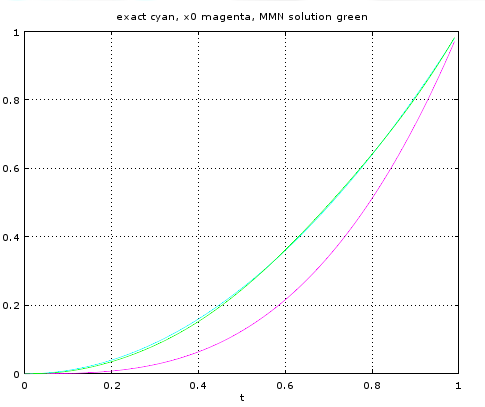
\includegraphics[height=6.0cm]{mmn_ch1}
	\caption{Восстановленное ММН решение.}
	\label{fig:mmn_ch1}
\end{figure}
Ниже в таблице \ref{table1.1} показаны результаты расчетов методами $\eqref{equ_rmn}$, $\eqref{equ_alphaproc}$, $\Delta=\frac{\|F(x^k)+\alpha(x^k-x^0)-y\|}{\|y\|}$ --- относительная норма невязки. 
\begin{table}[]
	\centering
	\caption{Результаты для правой части без шума}
	\label{table1.1}
	\begin{tabular}{|l|c|c|c|}
		\hline
	\textbf{Метод}                   & \multicolumn{1}{l|}{\textbf{Параметр шага, $\gamma$}} & \multicolumn{1}{l|}{\textbf{$\Delta$}} & \multicolumn{1}{l|}{\textbf{Число итераций, N}} \\ \hline
		ММО                              & \begin{tabular}[c]{@{}c@{}}0.5\end{tabular}                                       & 0.003                                   & 25                                     \\ \hline
		\multicolumn{1}{|r|}{ММО модиф.} & 0.5                                                                                                           & 0.003                                   & 22                                     \\ \hline
		МНС                              & 0.001                                                                                                         & 0.003                                   & 283                                    \\ \hline
		МНС модиф.                       & \begin{tabular}[c]{@{}c@{}}0.02 (c 0-й итер.), \\ 0.005 (c 30-й итер.),\\   0.002 (c 32-й итер.)\end{tabular} & 0.003                                   & 32                                     \\ \hline
		ММН                              & 1                                                                                                             & 0.003                                   & 32                                     \\ \hline
		ММН модиф.                       & 1                                                                                                             & 0.003                                   & 27                                     \\ \hline
		РМН                              & 1                                                                                                             & 0.003                                   & 26                                     \\ \hline
		РМН модиф.                       & \begin{tabular}[c]{@{}c@{}}0.75\end{tabular}                                       & 0.003                                   & 6                                      \\ \hline
	\end{tabular}
\end{table}

Выбор начального приближения, достаточно близкого к точному решению, обусловлен условиями теорем 1.1, 1.5 для сходимости немодифицированных вариантов методов $\eqref{equ_rmn}$, $\eqref{equ_alphaproc}$. Так же следует отметить, что теорема 1.5 не гарантирует, что при $\gamma=1$ итерационный процессы $\eqref{equ_alphaproc}$ будут сходиться, так же как и модифицированный вариант метода Ньютона. Поэтому сходимость некоторых этих методов в рамках эксперимента была достигнута при выборе $\gamma<1$, тогда как для метода Ньютона немодифицированного варианта сходимость при $\gamma=1$ доказана теоремой 1.1, что и подтверждается экспериментом. Для достижения необходимой точности решения модифицированным вариантом МНС параметр $\gamma$ потребовалось несколько раз уменьшать. С 30-й итерации $\gamma=0.005$, с 32-й итерации $\gamma=0.002$.

{\bfseries 1.3.2.} Эксперимент для задачи без использования шума с начальным приближением, далеким от точного решения.
Точное решение и правая часть такие же, как в эксперименте 1.3.1.  Начальное приближение $x^0(t)=0$, $\bar\alpha=\alpha=10^{-2}$, критерий останова $\frac{\|x^k-z\|}{\|z\|}\le\varepsilon=10^{-1}$, где $x^k$ --- приближение на $k$-й итерации. %%На рис.~\ref{fig:mmn_ch1_const} изображено восстановленное решение методом ММН. Точное решение отмечено голубым цветом, начальное приближение --- малиновым, ММН --- зеленым. 
%\begin{figure}
%	\centering
%	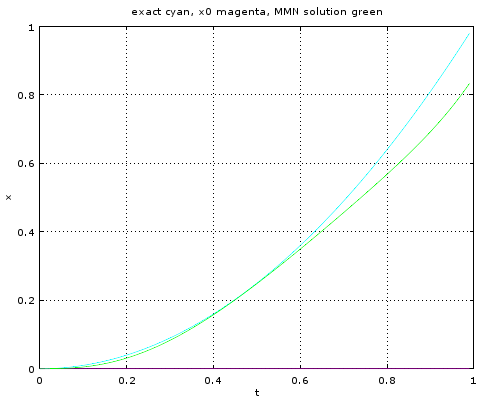
\includegraphics[height=6.0cm]{mmn_ch1_const}
%	\caption{Восстановленное ММН решение с нулевым начальным приближением.}
%	\label{fig:mmn_ch1_const}
%\end{figure}
Ниже в таблице \ref{table1.2} показаны результаты расчетов методами $\eqref{equ_rmn}$, $\eqref{equ_alphaproc}$, $\Delta$ --- относительная норма невязки. 
\begin{table}[]
	\centering
	\caption{Результаты для правой части без шума, с начальным приближением, равным константе}
	\label{table1.2}
	\begin{tabular}{|l|c|c|c|}
		\hline
		\textbf{Метод}                   & \multicolumn{1}{l|}{\textbf{Параметр шага, $\gamma$}} & \multicolumn{1}{l|}{\textbf{$\Delta$}} & \multicolumn{1}{l|}{\textbf{Число итераций, N}} \\ \hline
		ММО                              & 1                                                     & 0.015                                  & 25                                              \\ \hline
		\multicolumn{1}{|r|}{ММО модиф.} & 0.1                                                   & 0.015                                  & 20                                              \\ \hline
		МНС                              & 0.025                                                 & 0.021                                  & 27                                              \\ \hline
		МНС модиф.                       & 0.025                                                 & 0.024                                  & 24                                              \\ \hline
		ММН                              & 1                                                     & 0.019                                  & 12                                              \\ \hline
		ММН модиф.                       & 1                                                     & 0.016                                  & 8                                               \\ \hline
		РМН                              & 1                                                     & 0.016                                  & 19                                              \\ \hline
		РМН модиф.                       & 0.75                                                  & 0.016                                  & 8                                               \\ \hline
	\end{tabular}
\end{table}

Выбор начального приближения обусловлен фактом, установленным в статье \cite{Vasin_2016}, где для модифицированных вариантов методов $\eqref{equ_alphaproc}$ доказывается глобальная сходимость итерационных процессов. Для сходимости модифицированного метода Ньютона требование близкого начального приближения оговаривается в статье \cite{VasAkiMin2013}, но в данном случае была достигнута требуемая точность, как и для немодифицированных методов, рассматриваемых в данной главе. Факт сходимости при $\gamma=1$ не установлен для каждого из методов, однако при соответствующем $\gamma<1$ методы $\eqref{equ_rmn}$, $\eqref{equ_alphaproc}$ должны сходиться по теореме 1.5, этому не противоречат результаты расчетов.

{\bfseries 1.3.3.} Эксперимент для задачи с возмущенной правой частью с начальным приближением, далеким от точного решения.
Точное решение такое же, как в эксперименте 1.3.1. Правая часть $y^\delta(t)=y(t)e^{\frac{\delta}{5} sin(t/{\delta}^2)}$, $\delta=0.1$, $\|y-y^{\delta}\|=0.07<\delta$. Начальное приближение $x^0(t)=0$, $\bar\alpha=1$, $\alpha=10^{-3}$, критерий останова $\frac{\|x^k-z\|}{\|z\|}\le\varepsilon=0.25$, где $x^k$ --- приближение на $k$-й итерации. Ниже в таблице \ref{table1.3} приведены результаты расчетов.
\begin{table}[]
	\centering
	\caption{Результаты для задачи с шумом}
	\label{table1.3}
	\begin{tabular}{|l|c|c|c|}
		\hline
		\textbf{Метод}                   & \multicolumn{1}{l|}{\textbf{Параметр шага, $\gamma$}} & \multicolumn{1}{l|}{\textbf{$\Delta$}} & \multicolumn{1}{l|}{\textbf{Число итераций, N}} \\ \hline
		ММО                              & 1                                                     & 0.042                                  & 9                                               \\ \hline
		\multicolumn{1}{|r|}{ММО модиф.} & 1                                                     & 0.042                                  & 9                                               \\ \hline
		МНС                              & 1                                                     & 0.041                                  & 9                                               \\ \hline
		МНС модиф.                       & 1                                                     & 0.040                                  & 9                                               \\ \hline
		ММН                              & 1                                                     & 0.045                                  & 9                                               \\ \hline
		ММН модиф.                       & 1                                                     & 0.045                                  & 9                                               \\ \hline
		РМН                              & 1                                                     & 0.042                                  & 9                                               \\ \hline
		РМН модиф.                       & 1                                                     & 0.042                                  & 8                                               \\ \hline
	\end{tabular}
\end{table}

В статье \cite{VasSkur2017} приводятся оценки погрешности двухэтапного метода для $\|u^{\delta}-\hat{u}\|$ сверху ($u^{\delta}$ --- решение уравнения с возмущенной правой частью, $\hat{u}$ --- решение уравнения $\eqref{equ1}$), устанавливается сходимость $$\lim_{\delta\to 0}\|A(u_{\alpha(\delta)}^{\delta})-f_\delta\|=0,$$ при $\alpha(\delta)\to 0$, $\delta\to 0$. Для задачи с возмущенной правой частью удалось достигнуть точности $\varepsilon$, не превыщающую оценку для $\|u^{\delta}-\hat{u}\|$, относительная норма невязки $\Delta$ уменьшается с каждой итерацией.

%\section{Выводы к первой главе}